%%%%%%%%%%%%%%%%%%%%%%%%%%%%%%%%%%%%%%%%%%%%%%%%%%%%%%%%%%%%%%%%%%%%%%%%%%%%%%%%
%2345678901234567890123456789012345678901234567890123456789012345678901234567890
%        1         2         3         4         5         6         7         8

\documentclass[letterpaper, 10 pt, conference]{ieeeconf}  % Comment this line out if you need a4paper

%\documentclass[a4paper, 10pt, conference]{ieeeconf}      % Use this line for a4 paper

\IEEEoverridecommandlockouts                              % This command is only needed if 
                                                          % you want to use the \thanks command

\overrideIEEEmargins                                      % Needed to meet printer requirements.

% See the \addtolength command later in the file to balance the column lengths
% on the last page of the document

% The following packages can be found on http:\\www.ctan.org
%\usepackage{graphics} % for pdf, bitmapped graphics files
%\usepackage{epsfig} % for postscript graphics files
%\usepackage{mathptmx} % assumes new font selection scheme installed
%\usepackage{times} % assumes new font selection scheme installed
\usepackage{float}
\usepackage{ngerman}
\usepackage[utf8]{inputenc}
\usepackage{color}
\usepackage{amsmath}
\usepackage{bm}
\usepackage{amssymb}
\usepackage{graphicx}
\graphicspath{{./figures/}}
% Symbole für Tabelle: grüner Haken und rotes Kreuz
\newcommand{\ok}{{\color{green}\checkmark}}
\newcommand{\no}{{\color{red}$\boldsymbol\times$}}

\usepackage{calrsfs}
\DeclareMathAlphabet{\pazocal}{OMS}{zplm}{m}{n}
\newcommand{\body}[1]{\mathcal{B}_{#1}}
\newcommand{\ks}[1]{\mathcal{F}_{#1}}

\title{\LARGE \bf
Kinematics and Dynamics Model via explicit Elimination of Kinematic Constraints of an Exoskeleton for Craftsmen Force Assistance
}


\author{Moritz Schappler$^{1}$ and Sami Haddadin$^{2}$% <-this % stops a space
\thanks{*This work was supported by the German Federal Ministry of Education and Research under Grant no. 16SV6175}% <-this % stops a space
\thanks{$^{1}$Moritz Schappler
        {\tt\small schappler@irt.uni-hannover.de}}%
\thanks{$^{2}$Sami Haddadin
        {\tt\small haddadin@irt.uni-hannover.de}}%
}


\begin{document}



\maketitle
\thispagestyle{empty}
\pagestyle{empty}


%%%%%%%%%%%%%%%%%%%%%%%%%%%%%%%%%%%%%%%%%%%%%%%%%%%%%%%%%%%%%%%%%%%%%%%%%%%%%%%%
\begin{abstract}

abstract

\end{abstract}


%%%%%%%%%%%%%%%%%%%%%%%%%%%%%%%%%%%%%%%%%%%%%%%%%%%%%%%%%%%%%%%%%%%%%%%%%%%%%%%%
\section{Introduction and State of the Art}

Exoskeletons for assistance and rehabilitation

list different upper limb exoskeletons with different concepts

techniques and tools for kinematics and dynamics modeling

model assumptions for wearable robots: kinematic coupling of human and exoskeleton. Exoskeleton may contain passive joints (unlike serial chain robots), floating base assumption for base forces

contributions of the paper:
presentation of a novel exoskeleton mechanism designed
explicit kinematics and dynamics modeling for hybrid mechanism with gear and closed loop kinematic constraints
new approach for implementation of kinematic constraints in explicit form optimized for processing with computer algebra systems.

paper structured as follows: scenario and system presentation, detailed kinematics and dynamics model, control concepts for the system, simulation environment and simulation results.

\section{Exoskeleton and Scenario}

\subsection{Scenario}

force assistance for craftsmen
project goals \cite{NuelleSchTapLil2017}: 
* reduce fatigue of the worker and work-induced diseases, 
* increase work quality by projection of additional information (augmented reality, \cite{NuelleBriTapDem2018})
* guiding the user

This continues the work presented in \cite{PetereitAlbJerSch2012}. 
The waist-carried demonstrator was tested under aspects of ergonomics and workspace and failed. Thus a concept of upper limb exoskeletons proximal to the users body were developed.

\subsection{Exoskeleton}

The exoskeleton consists of several parts which will be introduced in short before being studied closer regarding kinematics and dynamics models.

\subsubsection{Main structure following the Human Arm}

With the attachment at the users upper body and at the hand of the user given with the constraint of neither blocking the users workspace nor sight, the main structure of the exoskeleton follows the arm of the user closely with similar degrees of freedom.

Fig.\,\ref{fig:KAS5_CAD} shows a CAD model of the complete exoskeleton to be carried in a right-hand configuration.


\begin{figure}[tb!]
    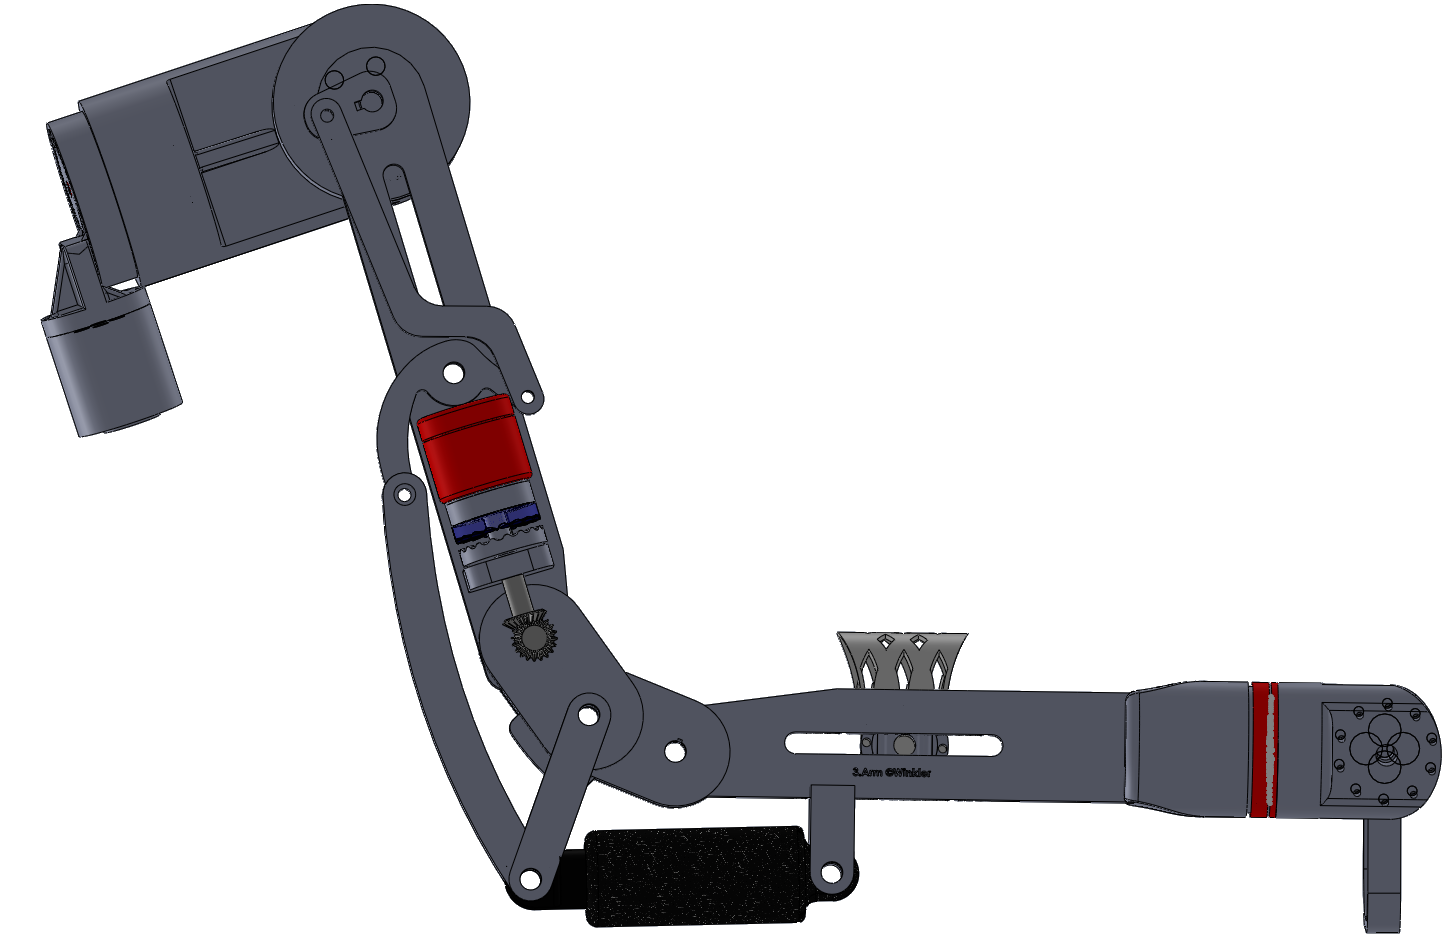
\includegraphics[width=\linewidth]{figures/KAS5_Seitenansicht_CAD_Ausschnitt_transp.png}
    \caption{CAD-Modell KAS5}
    \label{fig:KAS5_CAD}
\end{figure} 

\subsubsection{Three-Axis Elbow Joint}

The elbow joint of the mechanism is supposed to be on the axis of rotation of the users elbow.
To avoid constraint forces on the users elbow, the joint consists of three parallel axes which couple the upper and forearm via a central  through a gear wheel. The mechanism is shown in detail in Fig.\,\ref{fig:EllenbogenSimMech}.
The coupling mechanism connecting to the shoulder is left out for clarity.
The lever mechanism connecting the linear spring-damper-system with the elbow is fixed to the central elbow gear.

\begin{figure}[tb!]
    \begin{tabular}{c c c}
        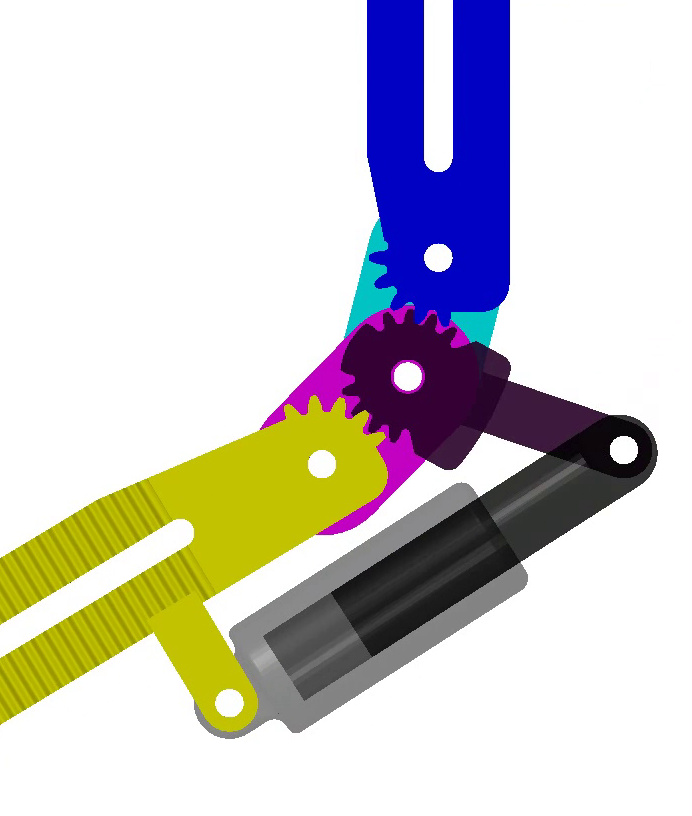
\includegraphics[width=0.28\linewidth]{figures/KAS6m3_SimMech_1.png} &
        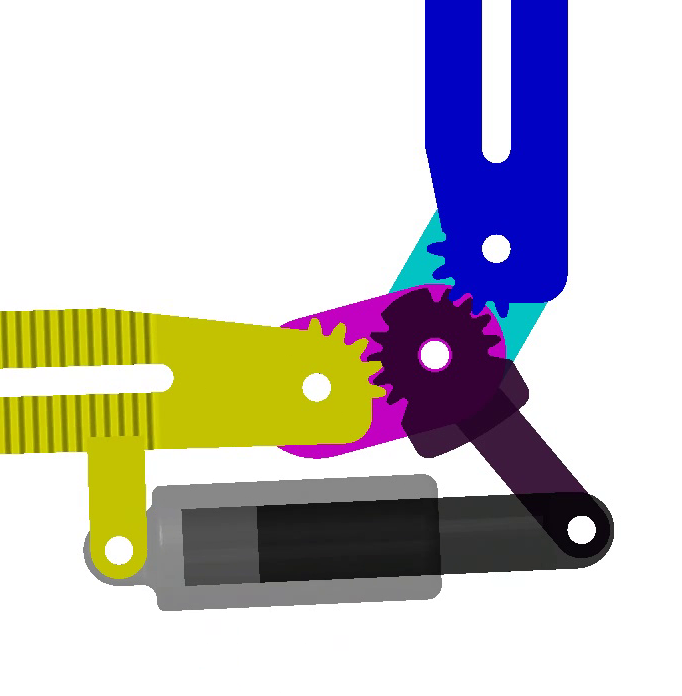
\includegraphics[width=0.30\linewidth]{figures/KAS6m3_SimMech_2.png} &
        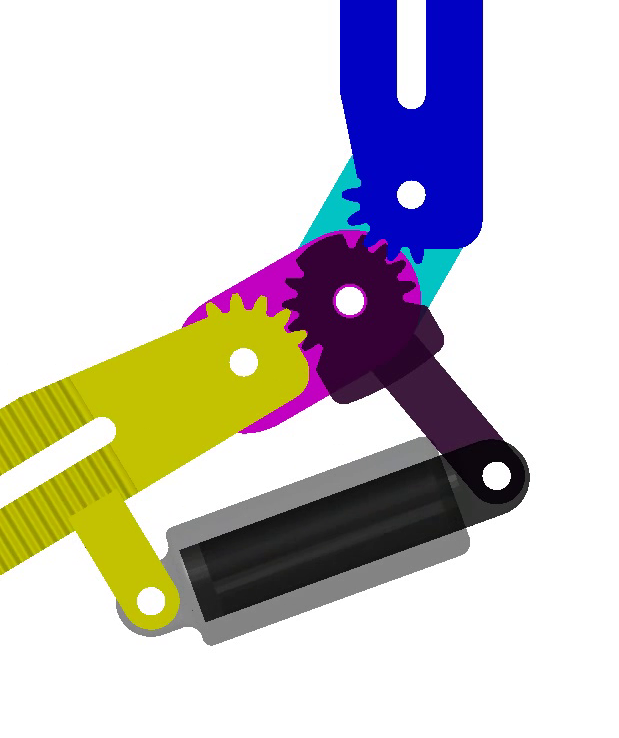
\includegraphics[width=0.28\linewidth]{figures/KAS6m3_SimMech_3.png}
    \end{tabular}

    \caption[Überprüfung der Kinematik in SimMechanics]{Überprüfung der Kinematik in SimMechanics am Beispiel unterschiedlicher Stellungen des KAS6. Damit lässt sich visuell ein korrektes Abrollen der Verzahnungen prüfen.}
    \label{fig:EllenbogenSimMech}
\end{figure} 

\subsubsection{Three-Axis Shoulder Joint}

The shoulder joint imitates the degrees of freedom of a simplified model of the human shoulder with three consecutive rotations with perpendicular axes.
The last axis of the shoulder joint corresponding to the shoulder flexion/extension is parallel to the axes of the elbow and coupling mechanism, leaving the greatest part of the joints in one axes to simplify manufacturing and kinematics modeling.

\subsubsection{Coupling Mechanism for From the Shoulder to the Elbow}

The shoulder F/E joint and the elbow joint are coupled via a mechanism consisting of two crank-lever-mechanisms.
This removes one degree of freedom of the system and forces the shoulder and first elbow rotation to move on a common trajectory.
With this coupling it is possible to transfer forces from the shoulder to the elbow and therefore move a motor actuating the elbow to the shoulder.
This concept is known from industrial robots with parallelogram structure connecting the second and third joint where moving the motor near the second joint reduces the inertia and gravitational load of the system.

\subsubsection{mechanical spring-damper system}

The elbow joint is connected via the central gear and a linear spring damper system with the forearm.
These spring systems are known e.\,g. for their use in mountain bikes.
The spring is transferring the moment created by the weight of the powertool towards the central gear.

\section{Kinematics and Dynamics Modelling}

\subsection{Kinematic Model}

All rotational axes of the mechanism are describes as single-DoF joints using the modified Denavit-Hartenberg notation from \cite{KhalilKle1986} to describe the position and orientation of the frames attached to all rigid bodies of the mechanism.
The parameters describing the transformations between these frames are given in Tab.\,\ref{tab:mdh_parameter}.
%
\begin{table}
    \begin{tabular}[t]{|c||c|c||c|c|c|c|c|}
        \hline
        $i$ & $\mu_i$ & $\sigma_i$ & $\alpha_i$ & $d_i$ & $\theta_i$ & $r_i$ & $a(i)$ \\
        \hline
        1 & $1$ & $0$ & $0$ & $0$ & $\rho_1-\pi/2$ & $l_1$ & 0 \\
        2 & $1$ & $0$ & $-\pi/2$ & $0$ & $\rho_2+\pi/2$ & $l_2$ & 1 \\
        3 & $0$ & $0$ & $\pi/2$ & $0$ & $\rho_3$ & $l_3$ & 2 \\
        4 & $1$ & $0$ & $0$ & $l_4$ & $\rho_4$ & $0$ & 3 \\
        5 & $1$ & $0$ & $0$ & $2l_{5}$ & $\rho_5$ & $0$ & 4 \\
        6 & $0$ & $0$ & $0$ & $2l_{6}$ & $\rho_6$ & $0$ & 5 \\
        7 & $1$ & $0$ & $\pi/2$ & $0$ & $\rho_7$ & $l_{7}$ & 6 \\
        8 & $0$ & $2$ & $\pi/2$ & $0$ & $\delta_{1}+\pi/2$ & $l_{3}$ & 2 \\
        9 & $0$ & $0$ & $0$ & $-l_{8}$ & $-\delta_{2}$ & $0$ & 8 \\
        10 & $0$ & $0$ & $0$ & $l_{9}$ & $-\delta_{3}$ & $0$ & 3 \\
        11 & $0$ & $0$ & $0$ & $l_{10}$ & $\pi-\delta_{4}$ & $0$ & 10 \\
        12 & $0$ & $0$ & $0$ & $2l_{5}$ & $\delta_{5}-\pi/2$ & $0$ & 4 \\
        13 & $0$ & $2$ & $0$ & $2l_{5}$ & $\delta_{6}-\pi/2$ & $0$ & 12 \\
        14 & $0$ & $0$ & $0$ & $0$ & $3\pi/2-\delta_{7}$ & $0$ & 13 \\
        15 & $0$ & $1$ & $\pi/2$ & $0$ & $0$ & $l_{\mathrm{F}}$ & 14 \\
        \hline
    \end{tabular}
    \label{tab:mdh_parameter}
    \caption{MDH parameters of the structure}
\end{table}
%
A kinematic sketch of the mechanism from Fig.\,\ref{fig:KAS5_CAD} is given in Fig.\,\ref{fig:KAS5_kinematik}.
%
\begin{figure}[tb]
    \tiny
    \begin{minipage}[t]{7.5cm}
        \vspace{0.2cm} % wird für bounding box des Bilds benötigt
        \input{./figures/KAS5_m3_skizze_kinematik_2_KS.pdf_tex}
    \end{minipage}
    
    \caption{Kinematikmodell und Skizze des KAS5 nach \cite{KhalilKle1986}. Starrkörper sind durch entsprechende eingekreiste Nummern (entspricht Tabellenspalte \glqq{}$i$\grqq{}) und körperfeste Koordinatensysteme gekennzeichnet. Die Körper 8, 9, 10, 11, 13 sind die Kurbeln und Hebel der Parallelstruktur}
    \label{fig:KAS5_kinematik}
\end{figure}

Due to the structure of the mechanism, the extended notation with antecessor index $a(i)$, joint type marker $\sigma_i$ (0 for rotational joint, 1 for prismatic, 2 for fixed connection) and actuation marker $\mu_i$ (0 for passive, 1 for active joint) are used.
The marker $\mu_i$ is set to 1 for the joints representing the generalized coordinates, regardless whether they are actuated or not.

The mechanism is regarded without the kinematic constraints by virtually cutting the loop-closing joints resulting in a tree structure.

The coordinates $\bm{q}$ of the single-DoF joints of this unconstrained system can according to \cite{NakamuraGho1989} be separated into the generalized coordinates
%
\begin{equation}
\bm{q}_1=\begin{pmatrix}\rho_1 & \rho_2 & \rho_4 & \rho_5 &\rho_7 \end{pmatrix}^\mathrm{T}
\end{equation}
%
and the dependant coordinates
%
\begin{equation}
\bm{q}_2=\begin{pmatrix}\rho_3 & \delta_2 & \delta_3 & \delta_4 & \delta_5 & \delta_7 \end{pmatrix}^\mathrm{T}.
\end{equation}
%
The joint coordinates of the main structure are denoted with $\rho$ and the coordinates of the parallel coupling and support mechanism with $\delta$.
%
In the following, the dependant coordinates are expressed in the explicit form
%
\begin{equation}
\bm{q}_2=\bm{f}(\bm{q}_1)
\end{equation}
%
as a function of the generalized coordinates $\bm{q}_1$.
This will be used to get determine the configuration of the complete system depending on the pose of the main structure and to generate dynamics equations for simulation and model based controllers.

\subsection{Elimination of Kinematic Constraints}

The kinematic constraints of the system originate from the rolling condition of the elbow gears and the closed loop constraints in the coupling mechanism.

\subsubsection{Elbow Joint}

The gear constraints in the elbow joint originate from two gear mechanisms on both sides of the central gear.
The elbow CAD view of Fig.\,\ref{fig:EllenbogenSimMech} is detailed as a kinematic sketch in Fig.\,\ref{fig:KAS5_elbow}.
%
\begin{figure}[htb]
    \small
    \begin{minipage}[t]{7.5cm}
        \vspace{0.2cm} % wird für bounding box des Bilds benötigt
        \input{./figures/KAS5_kinematik_ellenbogen.pdf_tex}
    \end{minipage}
    
    \caption{Kinematic sketch of the Elbow Joint. Numbers in circles denote the rigid bodies, $W_1$ to $W_4$ denote the momentary pitch points of the gears.}
    \label{fig:KAS5_elbow}
\end{figure}
%
The constraints remove two DoF from the rigid bodies involved:
The main structure looses the DoF in the last axis corresponding to coordinate $\rho_6$ and the central gear is dependent of the configuration of the main structure affecting the coordinate $\delta_5$.
%
Describing the velocity of the pitch points $W_1$ and $W_2$ of the gears of $\body{3}$ and $\body{12}$ in frame $\ks{4}$ with the assumption of no backlash leads to
%
\begin{align}
\bm{v}_{W_1} &= \bm{v}_{W_2} \\
\bm{v}_{3} +\bm{\omega}_{4,3} \times \bm{r}_{4,W_1} &= \bm{v}_{12} +\bm{\omega}_{4,12} \times \bm{r}_{12,W_2} \\
-l_{5}\dot{\rho}_4\bm{e}_y &= -l_{5}\dot{\delta}_5\bm{e}_y
\end{align}
%
and results in the kinematic relation
%
\begin{align}
\delta_5 = \rho_4.
\label{equ:delta5_explicit}
\end{align}
%
Similarly, the rolling condition of the central gear ($\body{12}$, $W_3$) with the forearm ($\body{6}$, $W_4$), expressed in frame $\ks{5}$, can be written as the velocity of the pitch points
%
\begin{align}
\bm{v}_{W_3} &= \bm{v}_{W_4} \\
\bm{v}_{12} +\bm{\omega}_{5,12} \times \bm{r}_{5,W_3} &= \bm{v}_{6} +\bm{\omega}_{5,6} \times \bm{r}_{6,W_4} \\
-(-\dot{\rho}_5+\dot{\delta}_5)\bm{e}_z \times l_5\bm{e}_x &= \dot{\rho}_6\bm{e}_z \times (-l_6)\bm{e}_x \\
(-\dot{\rho}_5+\dot{\delta}_5) l_5 \bm{e}_y &= -l_6 \dot{\rho}_6\bm{e}_y
\end{align}
%
which results in the relation
%
\begin{align}
\rho_6 = \rho_5 - \rho_4 + \delta_8,
\end{align}
%
where the integration constant $\delta_8$ corresponds to a gear offset, which allows taking into account a shifted assembly of the central gear $\body{12}$ and forearm $\body{6}$. This offset was assumed to zero in (\ref{equ:delta5_explicit}) forcing an assembly according to the kinematic sketch for the central gear relative to the upper arm $\body{3}$.


\subsubsection{elbow-shoulder-coupling}

define circles: geometrical method to solve the kinematic constraints for the closed loops
calculate intersection points of the two circles via quadratic equations 

iterative procedure (first circle, second circle)

\subsubsection{complete model}



Es muss nicht die explizite Lösung der Zwangsbedingungen aus (\ref{equ:ZB_explizit}) gefunden werden, sondern nur die explizite Form für 
%
\begin{align}
\mathrm{sin}(\bm{q}_2) =& \bm{f}_\mathrm{sin}(\bm{q}_1) \\
\mathrm{cos}(\bm{q}_2) =& \bm{f}_\mathrm{cos}(\bm{q}_1) \\
\dot{\bm{q}}_2 =& \bm{f}_\mathrm{diff}(\bm{q}_1,\dot{\bm{q}}_1).
\end{align}


\subsection{Kinematic Constraints in Implicit Form}



\subsection{Dynamics Model}

\label{sec:Lagrange2Elim}
%
Diese Form wird in den Energiegleichungen benötigt.
Vor der Elimination der ZB ist das Lagrange-Funktional $L$ in der Form
\begin{equation}
L(\bm{q},\dot{\bm{q}})=L(\mathrm{sin}(\bm{q}_1),\mathrm{cos}(\bm{q}_1),\dot{\bm{q}}_1,\mathrm{sin}(\bm{q}_2),\mathrm{cos}(\bm{q}_2),\dot{\bm{q}}_2).
\end{equation}
Nach der Substitution sind sie in der für Lagrange 2. Art geeigneten Form in Darstellung der Minimalkoordinaten $\bm{q}_1$
%
\begin{equation}
L(\bm{q}_1,\dot{\bm{q}}_1)=L(\mathrm{sin}(\bm{q}_1),\mathrm{cos}(\bm{q}_1),\dot{\bm{q}}_1,\bm{f}_\mathrm{sin}(\bm{q}_1),\bm{f}_\mathrm{cos}(\bm{q}_1), \bm{f}_\mathrm{diff}(\bm{q}_1,\dot{\bm{q}}_1)).
\end{equation}
%
Mit dem Lagrange-Formalismus
%
\begin{equation}
\frac{\mathrm{d}}{\mathrm{d}t}\frac{\partial L(\bm{q}_1,\dot{\bm{q}}_1)}{\partial \dot{\bm{q}}_1} - \frac{\partial L(\bm{q}_1,\dot{\bm{q}}_1)}{\partial \bm{q}_1} = \bm{\tau}^c_1,
\end{equation}
%
der auch in \cite{NakamuraGho1989} zur Herleitung von (\ref{equ:tau_Projektion}) benutzt wurde, folgt wieder die gesuchte Dynamik-Darstellung aus (\ref{equ:Dyn_MinKoord}).

%
%Für Newton-Euler bräuchte man noch $d^2(x)/dt^2=...$.
%Diese Formen sind effizienter zu berechnen als die explizite Form $x=...$ (auf die dann wieder $sin()$, $cos()$ angewendet würde).
Das wurde in \cite{WangGosselin1998} schon so gemacht. Dort aber nicht wirklich hervorgehoben.

\section{Control Concept}

joint torque based gravity compensation

\section{Simulation Environment}

forward dynamics
simulink model
human user as force/torque in free space for first evaluations
coupling with musculo-skeletal model \cite{KuehnHuSchHad2018}


\section{Simulation Results}

energy consistency

\begin{figure*}[tb!]
    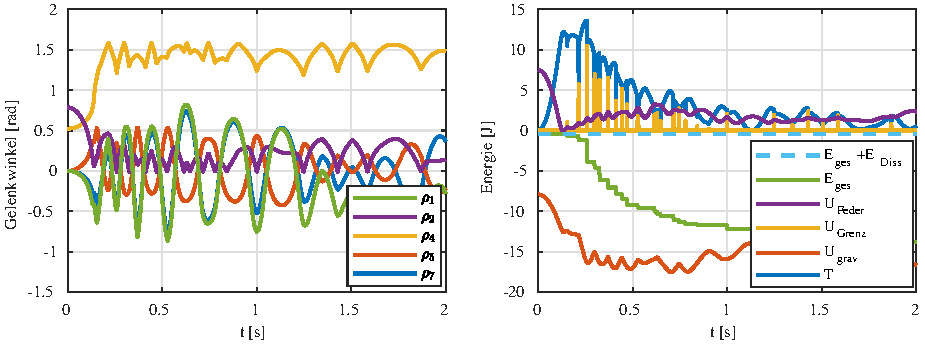
\includegraphics{figures/KAS5m5_Gelenkgrenzmodell_q_E.pdf} 
    \caption[Zeitverläufe aus der Simulation zur Prüfung der Energiekonsistenz]{Zeitverläufe aus der Simulation zur Prüfung der Energiekonsistenz. Links: Gelenkwinkel. Rechts: Energien (kinetische Energie $T$, Gravitationspotential $U_\mathrm{grav}$, Federenergie der modellierten Gelenkwinkelanschläge $U_\mathrm{Grenz}$, Federenergie der Linearfeder $U_\mathrm{Feder}$, Gesamtenergie $E_\mathrm{ges}$, Dissipierte Energie $E_\mathrm{Diss}$)}
    \label{fig:SimulationEnergiekonsistenz}
\end{figure*} 


improving gravity compensation

\section{Conclusions}

A conclusion.

\addtolength{\textheight}{-12cm}   % This command serves to balance the column lengths
                                  % on the last page of the document manually. It shortens
                                  % the textheight of the last page by a suitable amount.
                                  % This command does not take effect until the next page
                                  % so it should come on the page before the last. Make
                                  % sure that you do not shorten the textheight too much.

%%%%%%%%%%%%%%%%%%%%%%%%%%%%%%%%%%%%%%%%%%%%%%%%%%%%%%%%%%%%%%%%%%%%%%%%%%%%%%%%



%%%%%%%%%%%%%%%%%%%%%%%%%%%%%%%%%%%%%%%%%%%%%%%%%%%%%%%%%%%%%%%%%%%%%%%%%%%%%%%%



%%%%%%%%%%%%%%%%%%%%%%%%%%%%%%%%%%%%%%%%%%%%%%%%%%%%%%%%%%%%%%%%%%%%%%%%%%%%%%%%
%\section*{APPENDIX}
%
%Appendixes should appear before the acknowledgment.


\section*{ACKNOWLEDGMENT}

...


%%%%%%%%%%%%%%%%%%%%%%%%%%%%%%%%%%%%%%%%%%%%%%%%%%%%%%%%%%%%%%%%%%%%%%%%%%%%%%%%


% BIBLIOGRAPHY
\bibliographystyle{ieeetr}
\bibliography{ref}
\end{document}
